% Created by Jim Finnis
% Date Wed Feb 24 13:35:30 2021


\section{Introduction}
These notes provide some architectural details for PCOT to help
maintainers. I'll try to keep them up to date.

PCOT is based around a directed graph of nodes which perform
transformations of data. For this reason, the nodes are sometimes
called ``transforms'' and are represented by the \texttt{XForm} class
in the code.
Usually the data in question is an image, or rather an ``image cube'':
these have an arbitrary number of channels, not just the typical
RGB or greyscale. However, the data can be anything at all --- it depends
on the node. There is some typechecking when constructing the graph:
for exampel, you can't connect a ``rectangle'' output to an ``image'' input.
The entire application is shown in Fig.~\ref{app.png}. On the right
is a ``palette'' from which nodes can be selected to add to the graph,
while on the left
is an area which can show controls for each node in the graph, while
in the centre-right is the graph itself. This is shown in more detail
in Fig.~\ref{graph.png}.

\begin{figure}[ht]
\center
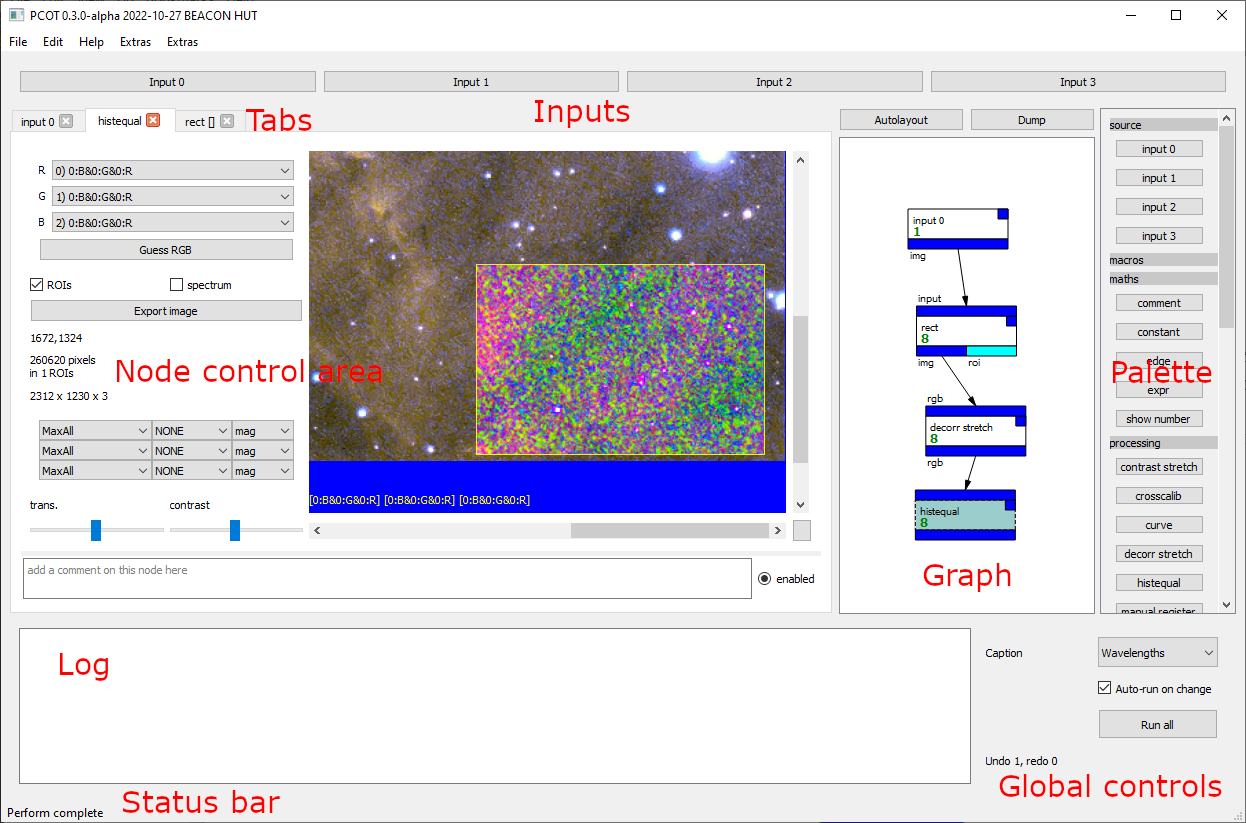
\includegraphics[width=5in]{app.png}
\caption{The PCOT application}
\label{app.png}
\end{figure}

\clearpage
This will take an RGB image from a file, perform a decorrelation stretch,
and then a histogram equalisation on the three channels. It will
only do this to a rectangular portion of the image (defined by the
\texttt{rect} node), annotating the region with some text defined in
the \texttt{rect} node's controls. The control region is currently
showing the output of the histogram equalisation.

\begin{figure}[ht]
\center
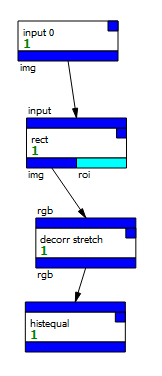
\includegraphics[width=1in]{graph.png}
\caption{An example graph}
\label{graph.png}
\end{figure}


\subsection{Notes on type checking}
Python is dynamically typed, but there are a lot of ``type annotations''
in the code. Unfortunately, Python's import rules mean there's also some
odd stuff going on. Annotations like
\begin{lstlisting}
class XFormType:
    ## @var name
    # name of the type
    name: str
    ## @var group
    # the palette group to which it belongs
    group: str
    ## @var ver
    # version number
    ver: str
    ## @var hasEnable
    # does it have an enable button?
\end{lstlisting}
are straightforward (and note the Doxygen annotations): we have three
string fields (\texttt{name}, \texttt{group} and \texttt{ver}) and
a boolean field (\texttt{hasEnable}). The next annotation, however,
is a link to a class defined further down the file, which in turn has
a field which is \texttt{XFormType}: a cyclic dependency. In such cases,
the standard PEP 0484 tactic is to use a string literal --- the type
checker will resolve this successfully and give appropriate warnings:
\begin{lstlisting}
    ## @var instances
    # all instances of this type in all graphs
    instances: List['XForm']
\end{lstlisting}
defines \texttt{instances} as a list of \texttt{XForm}.

Another oddity you may see in some of the files is this (from the top
of \texttt{xform.py} like the previous example):
\begin{lstlisting}
if TYPE_CHECKING:
    import graphscene
    import PyQt5.QtWidgets
\end{lstlisting}
These lines are only run when type checking, and are used to ensure
that appropriate classes are imported for type hints like this:
\begin{lstlisting}
    ## @var rect
    # the main rectangle for the node in the scene
    rect: ['graphscene.GMainRect']
    ## @var inrects
    # input connector rectangles
    inrects: List[Optional['graphscene.GConnectRect']]
    ## @var outrects
    # output connector rectangles
    outrects: List[Optional['graphscene.GConnectRect']]
    ## @var helpwin
    # an open help window, or None
    helpwin: Optional['PyQt5.QtWidgets.QMainWindow']
\end{lstlisting}
Without the \texttt{TYPE\_CHECKING} guard the program will not run, because
these imports are actually cyclic. However, they are only needed at 
compile time, so the \texttt{if}-statement is added to stop the import
at run time. Note the quotes: they are there to stop Python trying to
resolve the symbols at run time.

